\documentclass[12pt, titlepage]{article}


% Author's up-front packages
\usepackage[T1]{fontenc}
\usepackage[utf8]{inputenc}
\usepackage{longtable}

%Packages from template
\usepackage{amsmath, mathtools}
%\usepackage[round]{natbib}
\usepackage{amsfonts}
\usepackage{amssymb}
\usepackage{graphicx}
\usepackage{colortbl}
\usepackage{xr-hyper}
\usepackage{hyperref}
\usepackage{xfrac}
\usepackage{tabularx}
\usepackage{float}
\usepackage{siunitx}
\usepackage{booktabs}
\usepackage{multirow}
\usepackage[section]{placeins}
\usepackage{caption}
\usepackage{fullpage}

% Author's packages

\usepackage{cite}
\usepackage{indentfirst}
\usepackage{csquotes}
\usepackage{cleveref}

\hypersetup{
%bookmarks=true,     % show bookmarks bar?
colorlinks=true,       % false: boxed links; true: colored links
linkcolor=red,          % color of internal links (change box color with linkbordercolor)
citecolor=blue,      % color of links to bibliography
filecolor=magenta,  % color of file links
urlcolor=cyan          % color of external links
}

\usepackage{array}

%% Comments

\usepackage{color}

\newif\ifcomments\commentstrue

\ifcomments
\newcommand{\authornote}[3]{\textcolor{#1}{[#3 ---#2]}}
\newcommand{\todo}[1]{\textcolor{red}{[TODO: #1]}}
\else
\newcommand{\authornote}[3]{}
\newcommand{\todo}[1]{}
\fi

\newcommand{\wss}[1]{\authornote{blue}{SS}{#1}}
\newcommand{\an}[1]{\authornote{magenta}{Author}{#1}}


\newcommand{\progname}{STEM Moir{\'e} GPA}
\externaldocument[SRS:]{../SRS/SRS}
\externaldocument[TP:]{../TestPlan/TestPlan}
\externaldocument[MG:]{../Design/MG/MG}
\externaldocument[MIS:]{../Design/MIS/MIS}
\externaldocument[TP:]{../TestPlan/TestPlan}

%Set the custom referencing syste
	% Module
\newtheorem{M}{M}
\crefname{M}{M}{Ms}
	% Module Interface Specification
\newtheorem{MIS}{MIS}
\crefname{MIS}{MIS}{MISs}
	% Requirements
\newtheorem{R}{R}
\crefname{R}{R}{Rs}
	% Instance Model
\newtheorem{IM}{IM}
\crefname{IM}{IM}{IMs}
	% Test
\newtheorem{Test}{Test}
\crefname{Test}{Test}{Tests}
	% Theoretical Model
\newtheorem{T}{T}
\crefname{T}{T}{Ts}
	% Data Definition
\newtheorem{DD}{DD}
\crefname{DD}{DD}{DDs}
	% Test Report
\newtheorem{TestRep}{TestRep}
\crefname{TestRep}{TestRep}{TestReps}

\begin{document}

\title{Test Report: STEM Moir{\'e} GPA} 
\author{Alexandre Pofelski \\
		macid: pofelska \\
		github: slimpotatoes}
\date{\today}
	
\maketitle

\pagenumbering{roman}

\section{Revision History}

\begin{tabularx}{\textwidth}{p{3cm}p{2cm}X}
\toprule {\bf Date} & {\bf Version} & {\bf Notes}\\
\midrule
18/12/2017 & 1.0 & First incomplete version to meet deadline\\
\bottomrule
\end{tabularx}

~\newpage

\section{Symbols, Abbreviations and Acronyms}

The same Symbols, Abbreviations and Acronyms as in the SRS, the TestPlan, the 
MG and the MIS documents (available in 
\href{https://github.com/slimpotatoes/STEM_Moire_GPA}{\progname{}} repository) 
are used in the Test Report document. 

\newpage

\tableofcontents

\listoftables %if appropriate

\listoffigures %if appropriate

\newpage

\pagenumbering{arabic}

This document is providing information of \progname{} implementation by assessing the results of the tests designed in the TestPlan document. Regarding the size of \progname{} program, only a small part of the code has been tested in the required time frame therefore, only a few functional requirements have been evaluated. An important update to the document is planed once the implementation of the other tests are done.
\newline

For the moment, only a specific focus has been put on the \textbf{GPA Module} (\cref{MG:M_GPA} in the  MG document and \cref{MIS:MIS_GPA} in the MIS document) and the modules used by GPA which are:
\begin{itemize}
\item the \textbf{Data Structure Module} (\cref{MG:M_DataStruct} in MG document and \cref{MIS:MIS_DataStruct} in the MIS document)
\item the \textbf{Mask Module} (\cref{MG:M_Mask} in the MG document and \cref{MIS:MIS_Mask} in the MIS document)
\item the \textbf{Fourier Transform Module} (\cref{MG:M_FT} in MG document and \cref{MIS:MIS_FT} in the MIS document)
\item the \textbf{Gradient Module} (\cref{MG:M_Gradient} in MG document and \cref{MIS:MIS_Gradient} in the MIS document)
\item the \textbf{Phase Calculation Module} (\cref{MG:M_Phase} in MG document and \cref{MIS:MIS_Phase} in the MIS document)
\end{itemize}

\section{Functional Requirements Evaluation}

\subsection{\textbf{Test \cref{SRS:R_7} in \cref{SRS:IM_2}}: Correctness of the GPA method application}


\begin{TestRep}\normalfont\underline{{\cref{TP:T_Phase-Extraction-No-Strain} from TestPlan document}} \label{Test_Report_2} \newline

\cref{TP:T_Phase-Extraction-No-Strain} was designed to check if the gpa function of the GPA module outputs no strain with a simulated input signal with no strain. As a reminder, the GPA module is calculating $\Delta \overrightarrow{g}$ the variation of the wave vector $\overrightarrow{g}$ by isolating the spatial frequency $\overrightarrow{g}$ in Fourier space to extract the phase component. The variation of the phase is then related to the variation of the $\overrightarrow{g}$ wave vector using the gradient operation. \medskip

For \cref{TP:T_Phase-Extraction-No-Strain} to run, one SMH and the mask have to be provided. The SMH has been simulated using the numpy library by generating a 2D array of (256,256) in size with a single spatial frequency. Each element of the array (call pixel in the following of the document) represents the value of the sine function taken at the location of the array. The 2D array as a whole represents the sampled version of the 2D sine function and is a good representation of what is considered a STEM Moire hologram with a single frequency. The mask is set up to be centred on the simulated frequency of the Fourier transform of the SMH with a radius of one $\text{pixel}^{-1}$ (elementary unit in Fourier space). The mask array is performed by the function mask{\_}gaussian in the Mask Module. The maask{\_}gaussian function is executed inside the gpa function of the GPA module. \medskip

\Cref{fig:Test_2_explanation} is highlighting the results of \cref{TP:T_Phase-Extraction-No-Strain} for the particular case described below:
\begin{itemize}
\item $I_{SMH_{exp}}=\sin{(2\pi \overrightarrow{g}\cdot\overrightarrow{r})}$, with $\overrightarrow{g} = \frac{1}{16} \ \overrightarrow{u_x} \ \text{pixel}^{-1}$ which represents a periodicity of 16 pixels in the horizontal direction of $I_{SMH_{exp}}$. 
\item Mask $M$ of one $\text{pixel}^{-1}$ in radius and centred on $\overrightarrow{g}=(g_x,g_y)$ in $\widetilde{I}_{SMH_{exp}}$
\item $\overrightarrow{g} = \overrightarrow{g_\text{ref}} + \overrightarrow{\Delta g}$. Since $\overrightarrow{g}$ is constant and $\overrightarrow{g_\text{ref}}$ represents the value of $\overrightarrow{g}$ at a chosen pixel, $\overrightarrow{\Delta g} = \overrightarrow{0}$ everywhere in $I_{SMH_{exp}}=\sin{(2\pi g)}$ (case of no strain).
\end{itemize}

A visual summary of the test case can be read in \cref{fig:Test_2_explanation}. The I{\_}SMH plot is the representation of $I_{SMH_{exp}}$ and the Fourier Transform of I{\_}SMH plot is showing the location of $\overrightarrow{g}$ in Fourier space (maximum intensity) where the mask $M$ is positioned. The Raw Phase plot is highlighting the result of the GPA algorithm corresponding to the phase component related to the spatial frequency $\overrightarrow{g}$ and the Phase corrected plot is displaying the variation of the related to the spatial frequency $\overrightarrow{g}$. The vertical and horizontal components of $\overrightarrow{\Delta g}$ showing the gradient of the phase corrected and are related to the variation of the wave vector $\overrightarrow{g}$. More details can be found in the SRS document (\cref{SRS:T_2} and \cref{SRS:DD_2}).

\begin{figure}[H]
\begin{center}
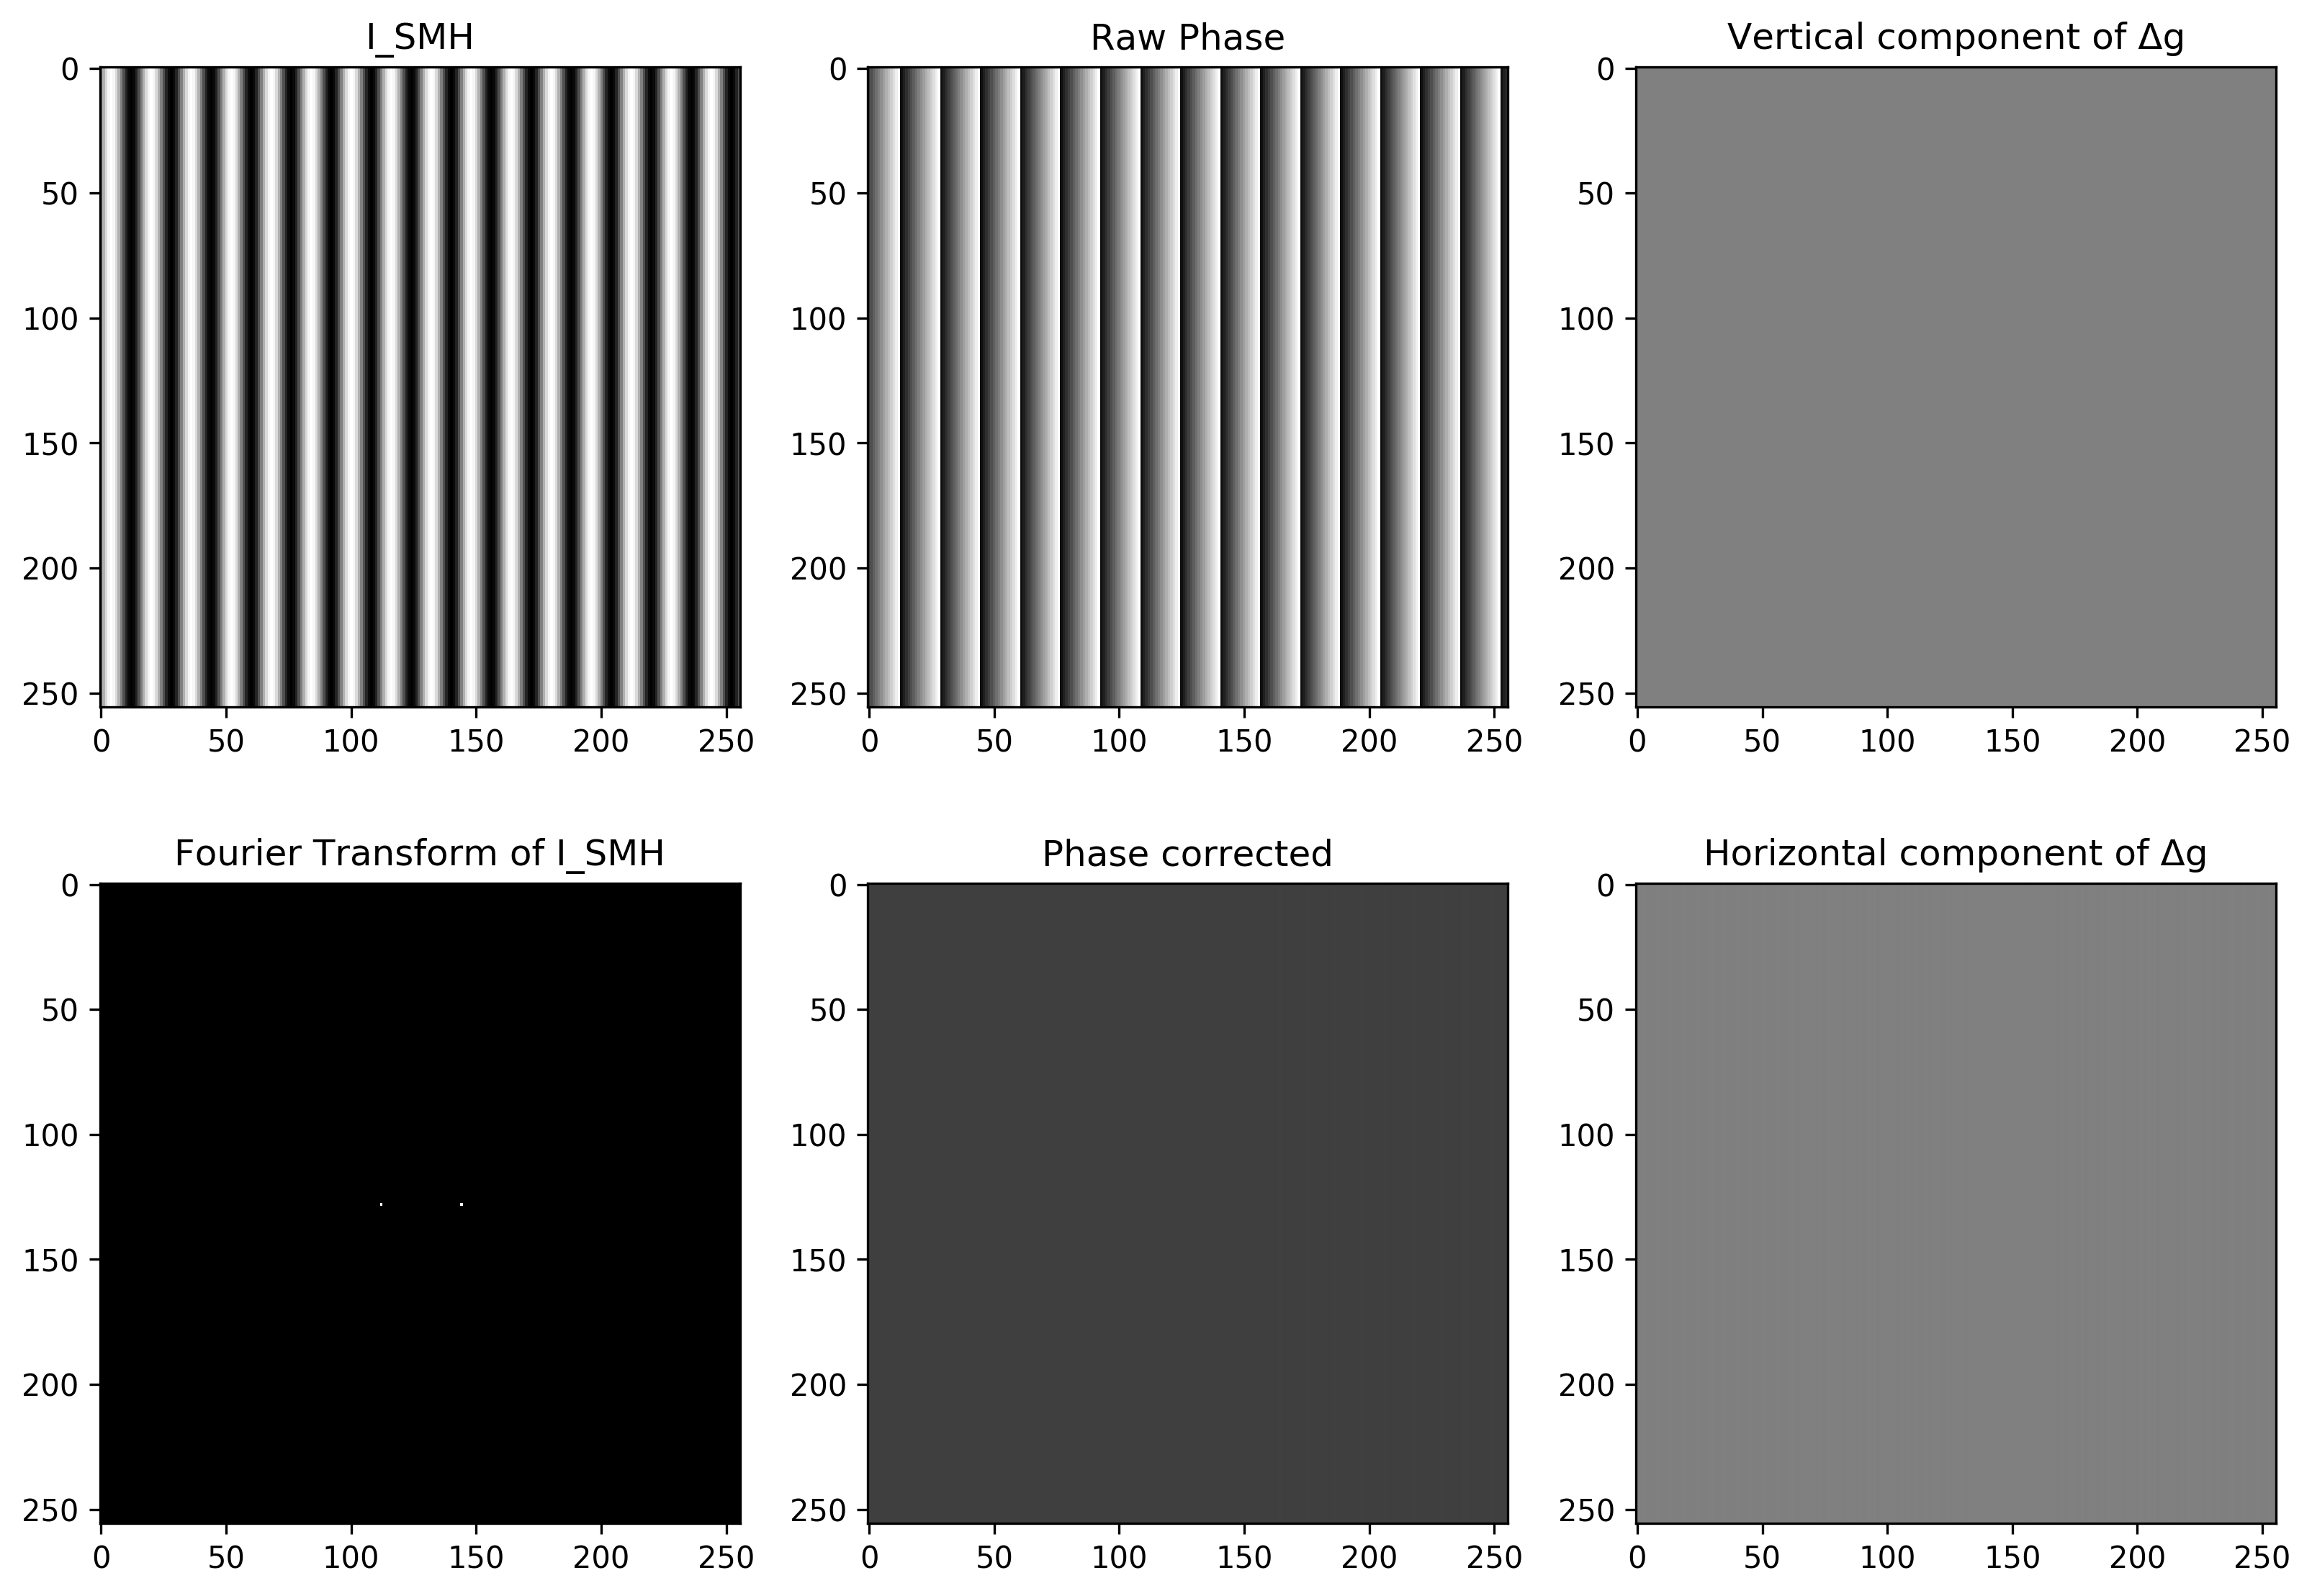
\includegraphics[scale=0.5]{Figures/Test_2_explanation.png}
\caption{Visual representation of one test case for \cref{Test_Report_2}}
\label{fig:Test_2_explanation}
\end{center}
\end{figure}

The expected output is $\overrightarrow{\Delta g} = \overrightarrow{0}$ on each pixel of the array. Since $\overrightarrow{\Delta g}$ is a 2D vector, the horizontal and the vertical components of the vector are shown on each pixel of the array to form the output test images (top and bottom figures on the left side of \cref{fig:Test_2_explanation}). For the intermediate variables, the phase corrected is expected to be constant, the raw phase to show a sawtooth shape with a constant slope along the horizontal direction. For the initial variables, $I_{SMH_{exp}}$ is a sampled version of a sine function and its Fourier transform should be two delta functions at the frequency $\overrightarrow{g}$ and $-\overrightarrow{g}$. Since the test case is only simulating a frequency in the horizontal direction, all the arrays from \cref{fig:Test_2_explanation} can be sliced by extracting only the results from a single vertical array. Such transformation is performed in \cref{fig:Test_2_explaination_1D}. The 1D representation helps in visualizing the different variables of the test case. 

\begin{figure}[H]
\begin{center}
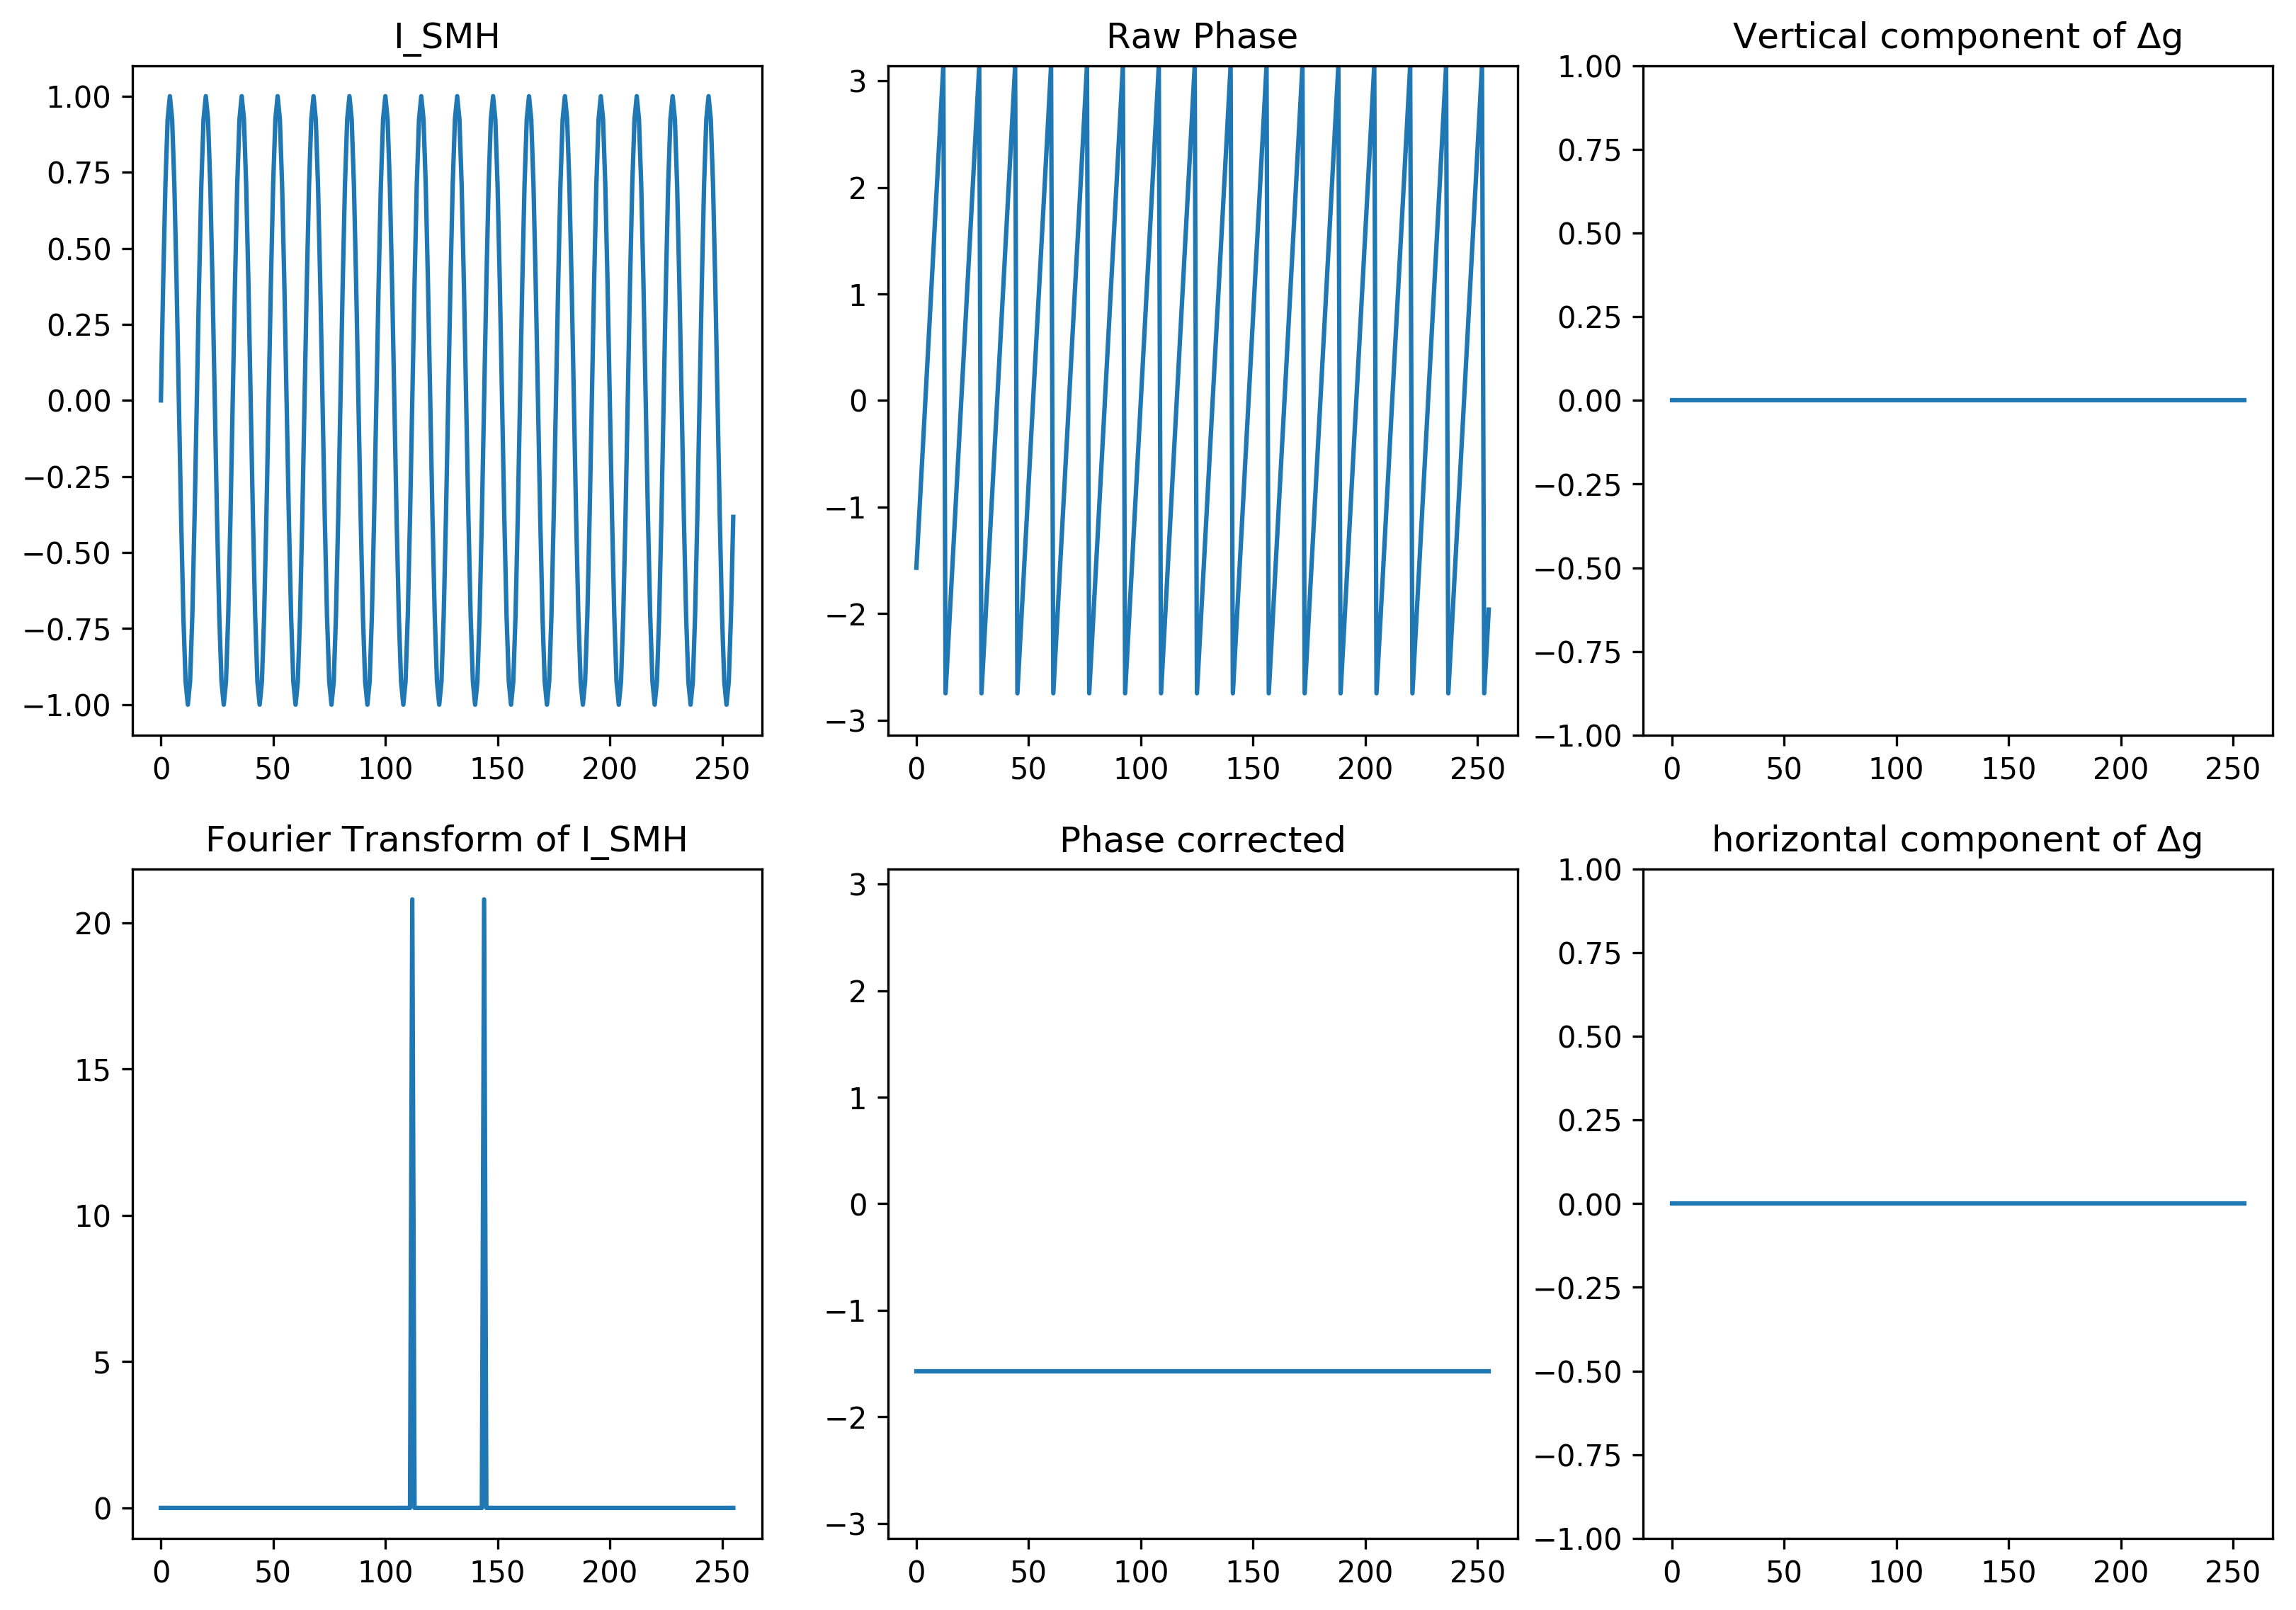
\includegraphics[scale=0.5]{Figures/Test_2_explanation_1D.png}
\caption{1D visual representation of one test case for \cref{Test_Report_2}}
\label{fig:Test_2_explaination_1D}
\end{center}
\end{figure}

The test can be summarized with the following metrics:
\begin{itemize}
\item Statistical \textbf{mean} of the elements part of horizontal line profile $\overrightarrow{\Delta g}$
\item Statistical \textbf{standard deviation} of the elements part of the horizontal line profile $\overrightarrow{\Delta g}$
\end{itemize}

For the test case described in \cref{fig:Test_2_explaination_1D}, the metrics are provided in \cref{tb:Metric_test_2_single_case}

\begin{table}[H]
\centering
\begin{tabular}{|c|c|c|}
\hline
$\overrightarrow{g} \ \text{(pixel)}^{-1}$ & Mean horizontal $\overrightarrow{\Delta g} \ \text{(pixel)}^{-1}$ & StDev horizontal $\overrightarrow{\Delta g} \ \text{(pixel)}^{-1}$ \\
\hline
16			& -2.2768245622195593e-18 & 3.2869874402072343e-16 \\ \hline
\end{tabular}
\caption{Table of metrics for one test case for \cref{Test_Report_2}}\label{tb:Metric_test_2_single_case}
\end{table}

It is reasonable to conclude that the errors are relatively small and can be considered negligible. The behaviour of the gpa function in the GPA module seems to be satisfactory. To check a more variety of test cases similar $I_{SMH_{exp}}$ with different periodicities were also tested. The following different periodicities are proposed: 3, 4, 4.1, 4.2, 4.5, 16 and 100 pixels. For each case, the appropriate mask is used and the radius of the mask is kept to 1 $\text{pixel}^{-1}$. The different test cases are summarized in \cref{fig:Test_2_Test_cases}. 

\begin{figure}[H]
\begin{center}
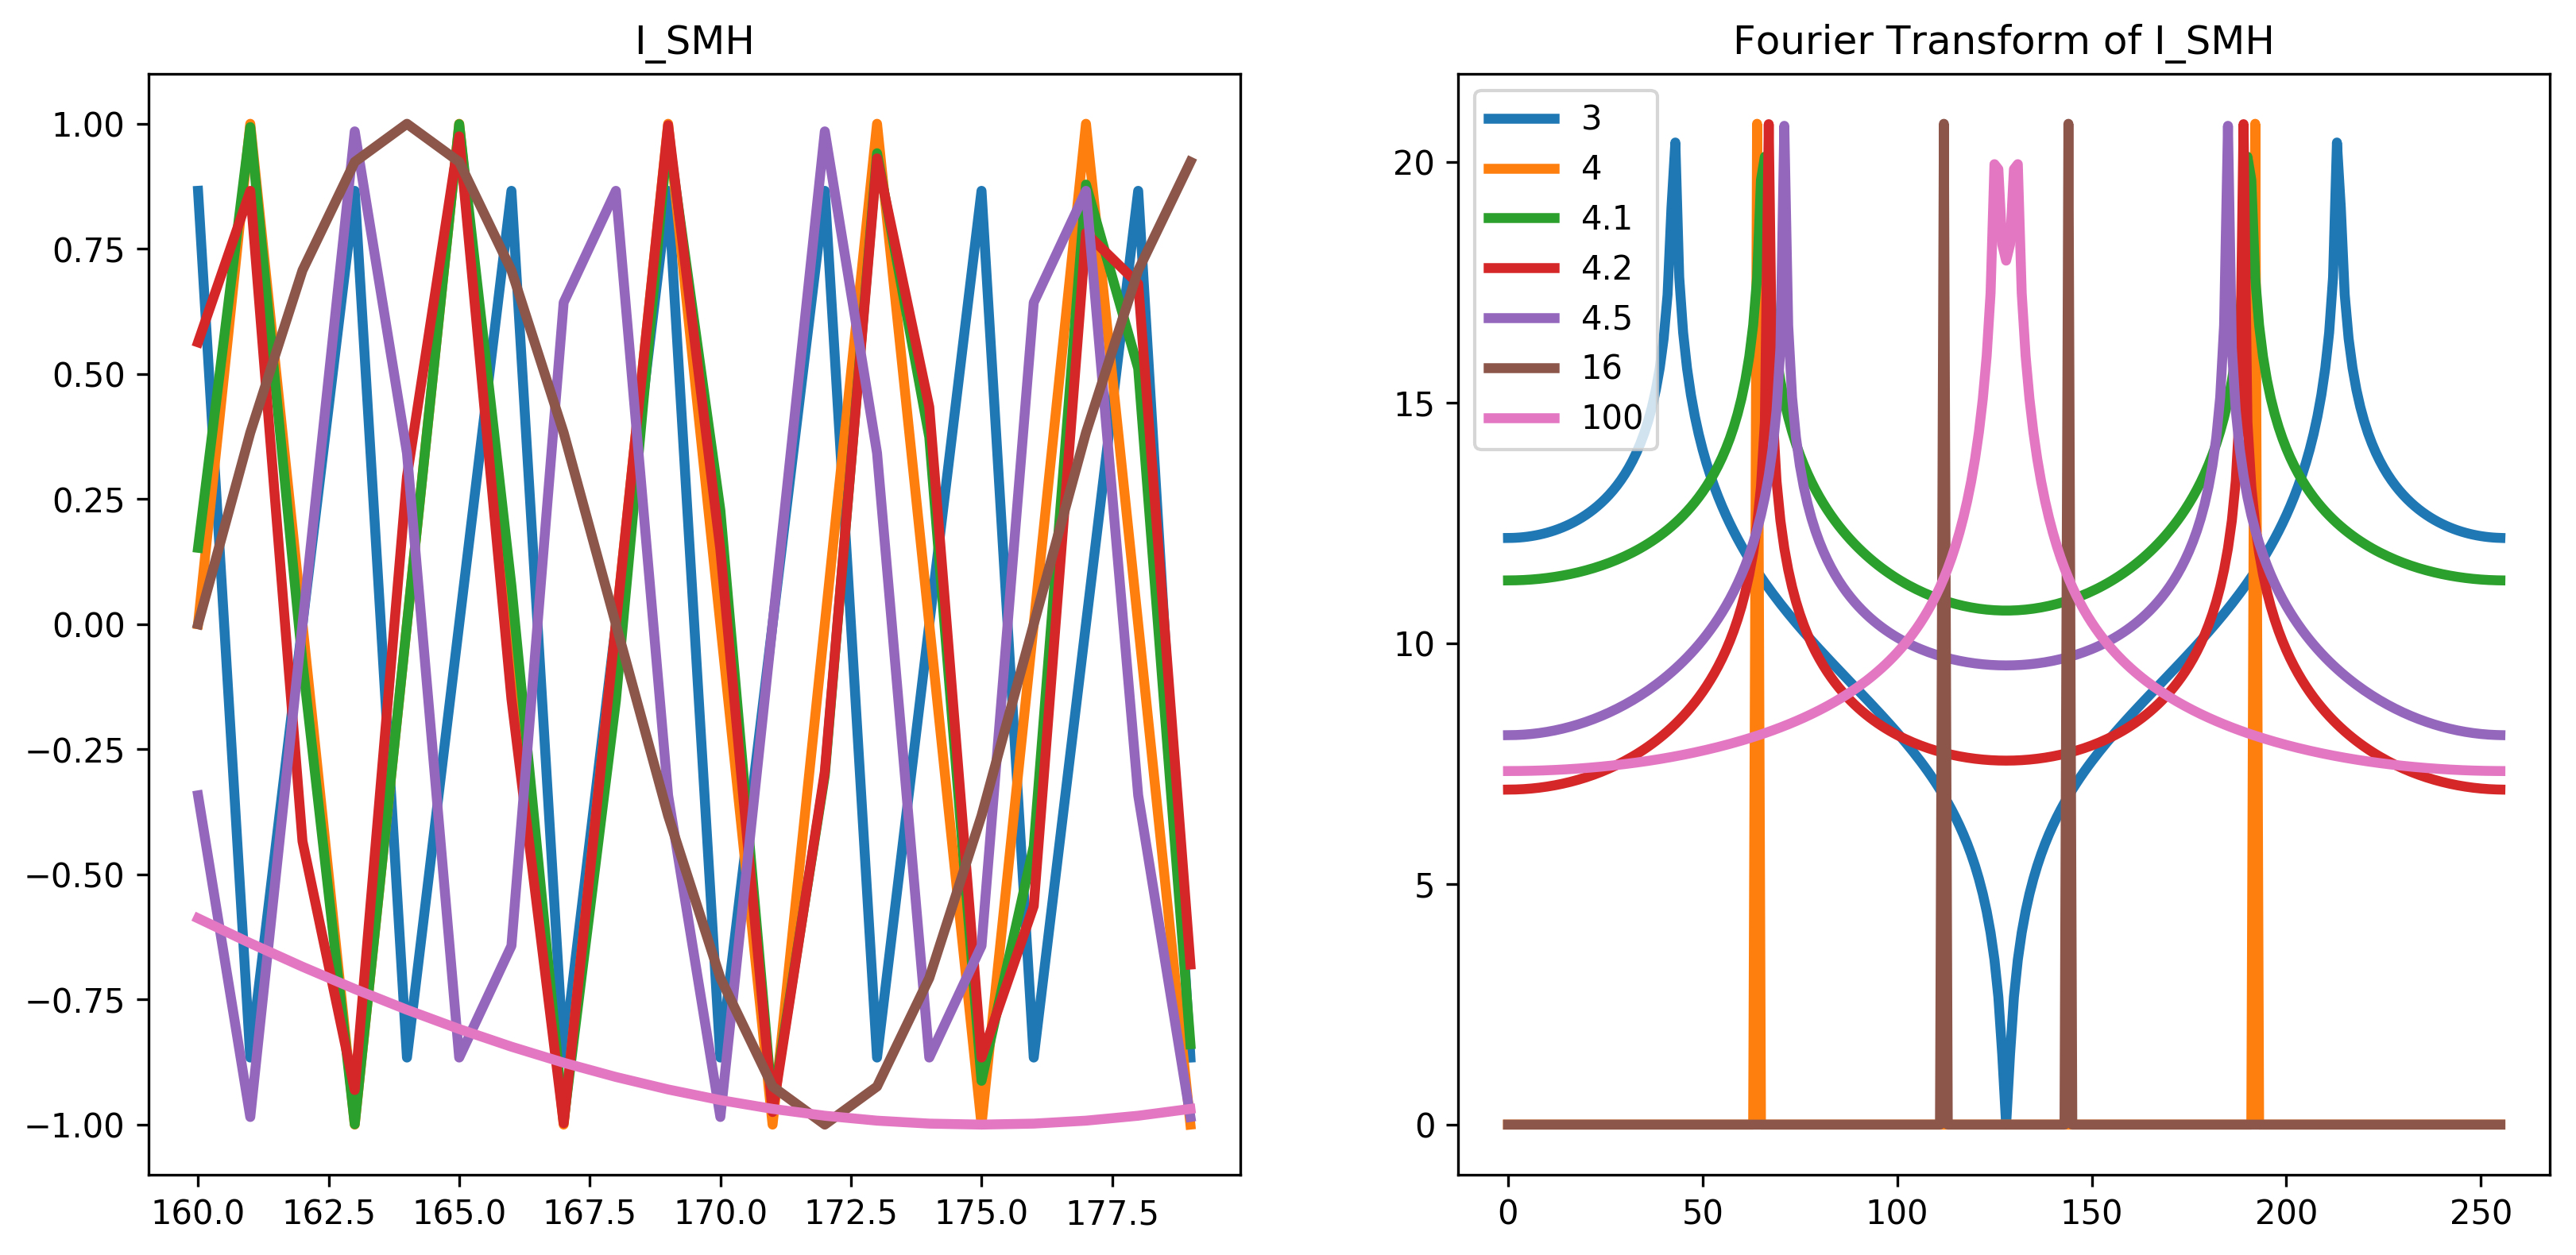
\includegraphics[scale=0.5]{Figures/Test_2_test_cases.png}
\caption{1D visual representation of the multiple test cases used for \cref{Test_Report_2}}
\label{fig:Test_2_Test_cases}
\end{center}
\end{figure}

The difference between the different periodicities in the Fourier transform plot can be commented. Only the particular cases with a periodicity of 4 and 16 pixels are highlighting a sharp delta function shape signal at their respective frequency. On all the other cases, the Fourier transform signal is spread on a range of frequency with a maximum at their respective frequency. The cause of the frequency spreading is for the moment unclear. It could be a mix between a sampling artifact and erros from the fast fourier transform algorithm. Those errors are not included in the model described in the SRS document and will have an effect on the gpa algorithm since some artificial frequencies seem to be present in the signal. However, those artifact are still weaker than the main signal coming from periodicity simulated.\medskip

The results of the test is highlighted in \cref{fig:Test_2_Test_results}. It is interesting to notice that some non negligible effects are now visible with specific test cases. It is difficult to assess if the numbers shown will have a significant impact on the final strain maps but the variation of the phase (translated into variation of $\overrightarrow{\Delta g}$) will contribute by adding noise in the signal.

\begin{figure}[H]
\begin{center}
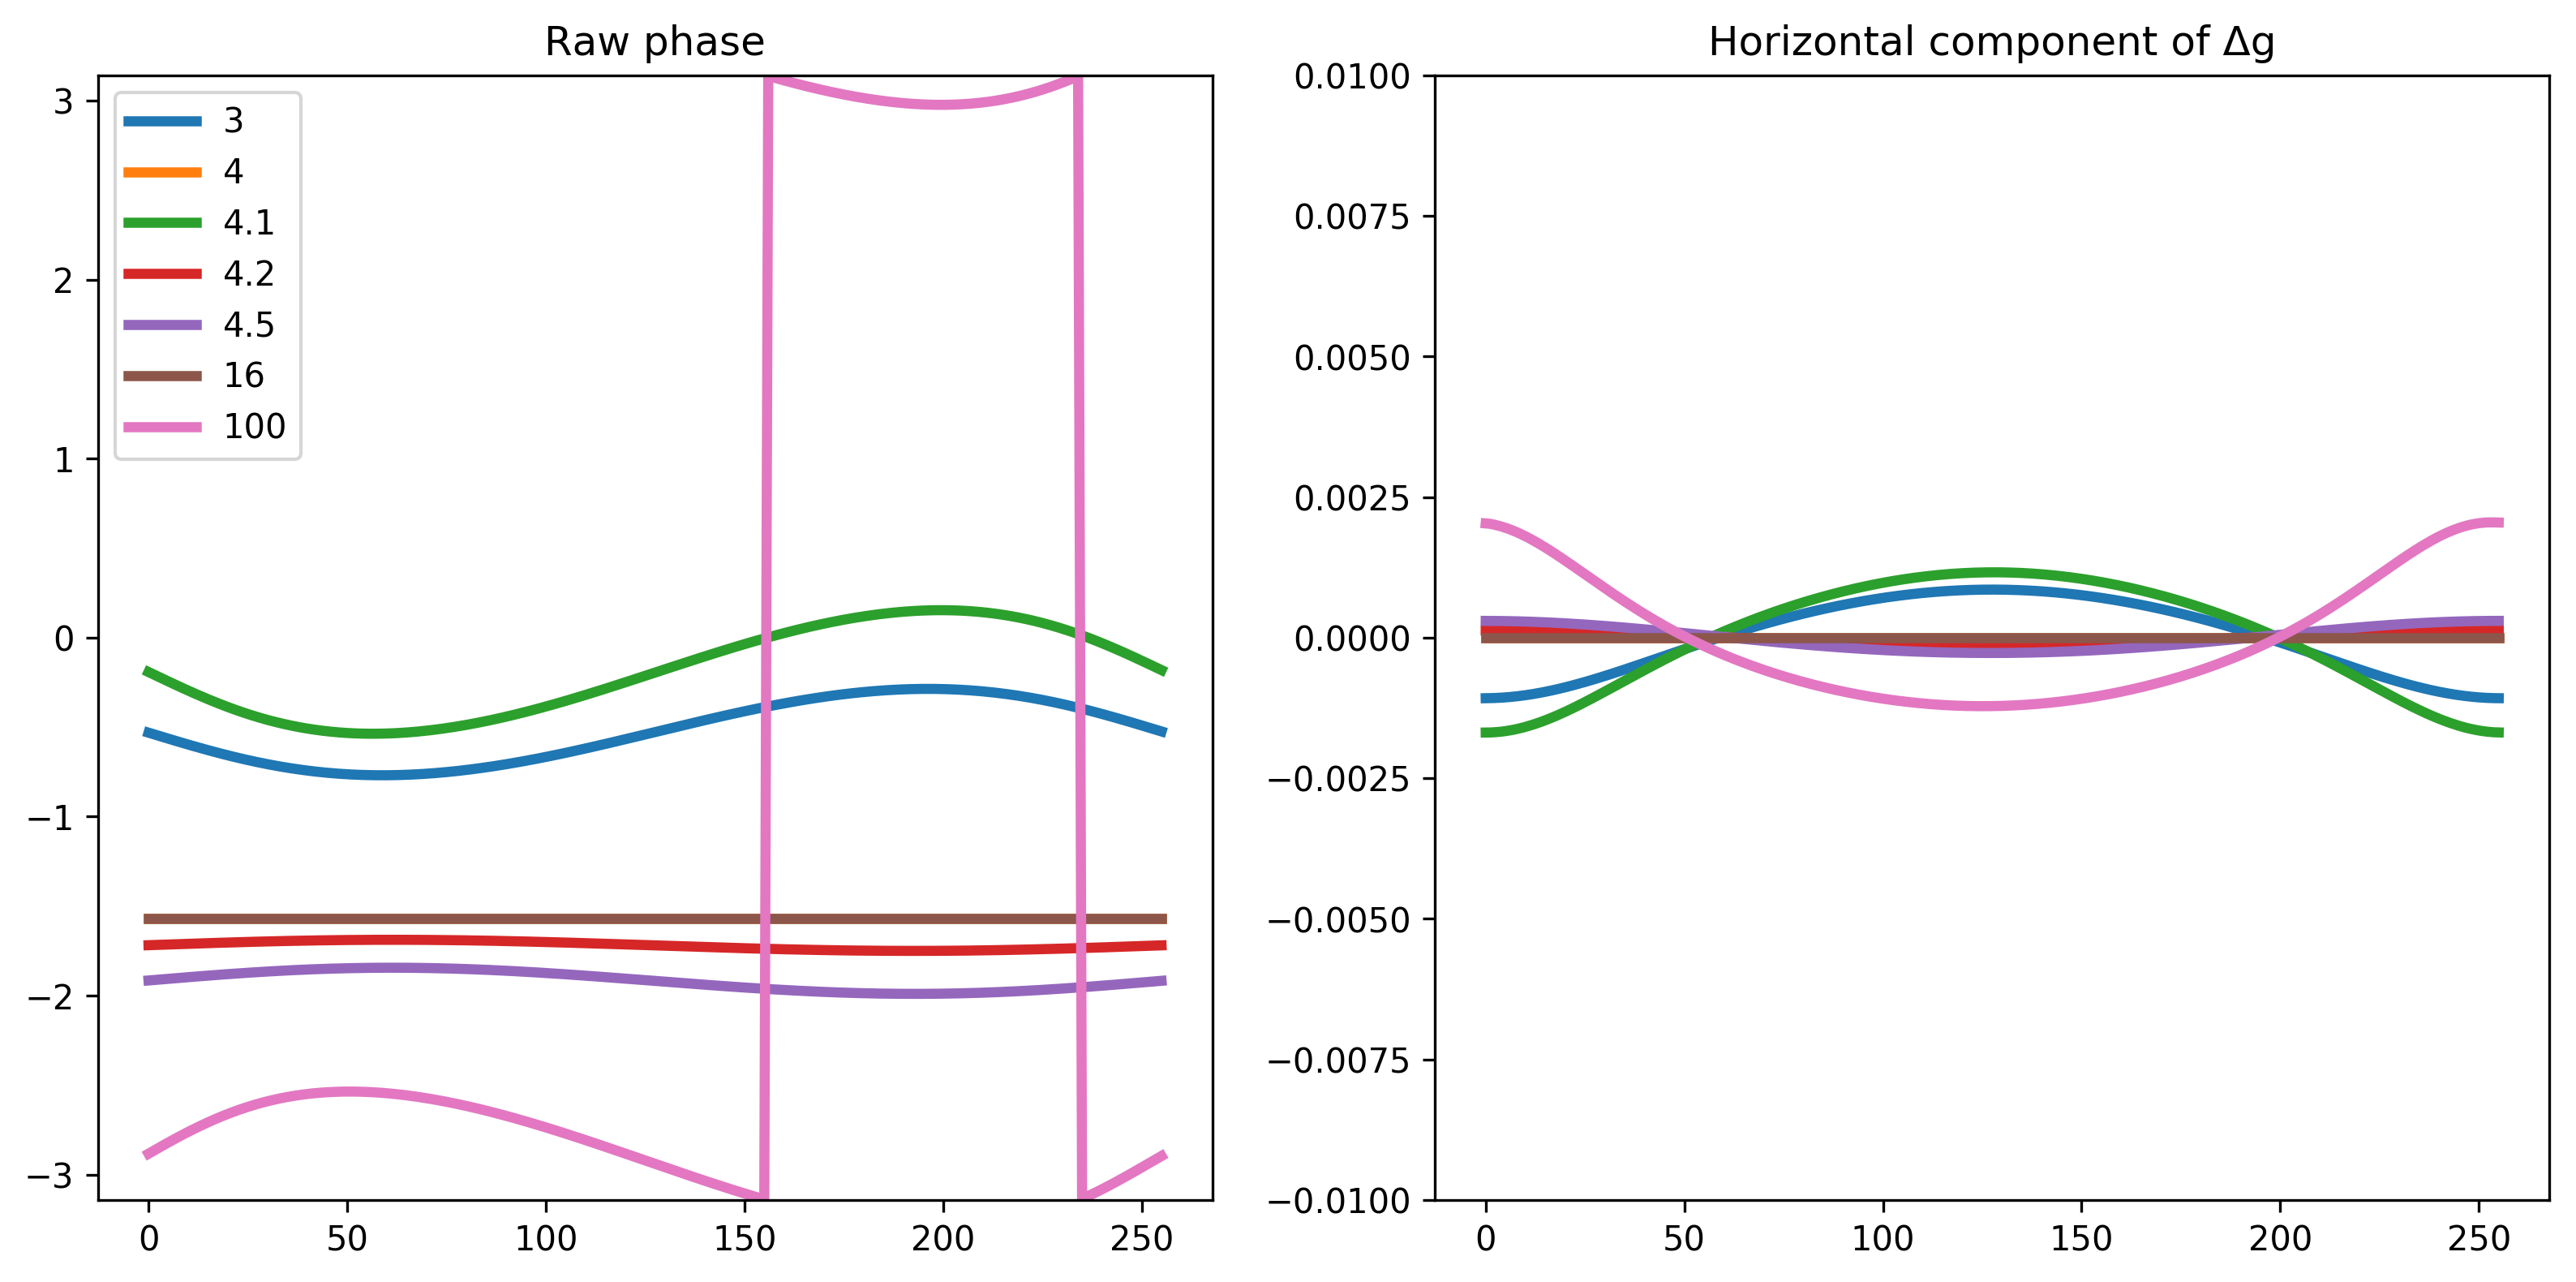
\includegraphics[scale=0.5]{Figures/Test_2_test_results.png}
\caption{1D visual representation of the test results for \cref{Test_Report_2}}
\label{fig:Test_2_Test_results}
\end{center}
\end{figure}

The table of metrics for all the cases is shown in \cref{tb:Metric_test_2_multiple_cases}. Those metrics might not be the most appropriate ones to assess GPA performance since the statistics remove the location where the error are minimized or maximized. The error distribution provided by the plot (or the image) are still needed to judge better the precision of the module. The error plot is provided in \cref{fig:Test_2_Test_error} and corresponds to the absolute value of horizontal component of $\overrightarrow{\Delta g}$ in \cref{fig:Test_2_Test_results}.

\begin{table}[H]
\centering
\begin{tabular}{|c|c|c|}
\hline
$\overrightarrow{g} \ \text{(pixel)}^{-1}$ & Mean horizontal $\overrightarrow{\Delta g} \ \text{(pixel)}^{-1}$ & StDev horizontal $\overrightarrow{\Delta g} \ \text{(pixel)}^{-1}$ \\
\hline
3 & 1.9414415841027127e-09 & 0.0006730746894985686 \\ \hline
\cellcolor{green} 4	 & \cellcolor{green} -9.540979117872439e-18 & \cellcolor{green} 7.341002270163171e-16 \\ \hline
\cellcolor[rgb]{1,0.8,0} 4.1 & \cellcolor[rgb]{1,0.8,0} 4.0351392667763858e-09 & \cellcolor[rgb]{1,0.8,0} 0.0009728477395757706 \\ \hline
4.2	& -1.6333255180214085e-10 & 8.581046509119554e-05 \\ \hline
4.5	& -3.9869652219449991e-10 & 0.0002022207376045426 \\ \hline
\cellcolor{green} 16 & \cellcolor{green} -2.2768245622195593e-18 & \cellcolor{green} 3.2869874402072343e-16 \\ \hline
\cellcolor[rgb]{1,0.8,0} 100 & \cellcolor[rgb]{1,0.8,0} -6.0785148749668448e-09 & \cellcolor[rgb]{1,0.8,0} 0.0010974597065239072 \\ \hline
\end{tabular}
\caption{Table of metrics for the test cases used for \cref{Test_Report_2}}\label{tb:Metric_test_2_multiple_cases}
\end{table}

\begin{figure}[H]
\begin{center}
\includegraphics[scale=0.5]{Figures/Test_2_test_error.png}
\caption{1D representation of the error measured for all the cases tested in \cref{Test_Report_2}}
\label{fig:Test_2_Test_error}
\end{center}
\end{figure}

Based on the error plot in \cref{fig:Test_2_Test_error}, the behaviour of the gpa module is not fully satisfactory. Potentially, the error could be small enough to be negligible however, \textbf{\cref{TP:T_Phase-Extraction-No-Strain}} is the simplest test case possible based on generated data. Noise and other artifacts will be included in the experimental data which could also contribute to the error. A system test on the whole program might help in assessing if the errors visible in GPA module have a significant impact on the deformation maps. \bigskip
\end{TestRep}

\begin{TestRep}\normalfont\underline{{\cref{TP:T_Phase-Extraction-Known-Strain}} from TestPlan document} \label{Test_Report_3} \newline

The same protocol as in \cref{Test_Report_2} has been used to generate the test cases of\cref{TP:T_Phase-Extraction-Known-Strain}. The only difference is that the generated data need to have a known strain in an area of the image. For simplicity, the left half of the image has been decided to be the reference state and the right half to be the strained state. An example of test case is shown in \cref{fig:Test_3_explanation} with the left side begin modelled by a sin function with a periodicity of 4 pixels and the right side modelled by a sin function with a periodicity of 4.5 pixels. The difference of periodicity correspond to the simulated strain field present on the right side of the image.\medskip

The details of the inputs used for test restuls shown in \cref{fig:Test_3_explanation} are  described below:
\begin{itemize}
\item $I_{SMH_{exp}}=\sin{(2\pi \overrightarrow{g}\cdot\overrightarrow{r} + \overrightarrow{K(x)}\cdot\overrightarrow{r})}$, with:
	\begin{itemize}
	\item $\overrightarrow{g} = \frac{1}{4} \overrightarrow{u_x} \ \text{pixel}^{-1}$ which represents a periodicity of 4 pixels in the horizontal direction of $I_{SMH_{exp}}$.
	\item $\overrightarrow{K(x)}$ such that $\begin{cases}
	\overrightarrow{K(x)}=\overrightarrow{0}, \ 0\leq x\leq127 \\
	\overrightarrow{K(x)}=\frac{4\times4.5}{4.5-4} \ \overrightarrow{u_x} \ \text{pixel}^{-1}, \ 128\leq x\leq 255
	\end{cases}$
	\end{itemize}
\item Mask $M$ of $20 \ \text{pixel}^{-1}$ in radius and centred on $\overrightarrow{g}=(g_x,g_y)$ (the unstrained frequency) in $\widetilde{I}_{SMH_{exp}}$
\item $\overrightarrow{g} = \overrightarrow{g_\text{ref}} + \overrightarrow{\Delta g}$. On the left side, $\overrightarrow{\Delta g} = \overrightarrow{0}$ and on the right side, $\overrightarrow{\Delta g} = (\frac{1}{4.5}-\frac{1}{4})\overrightarrow{u_x} + 0 \overrightarrow{u_y}$.
\end{itemize}

\begin{figure}[H]
\begin{center}
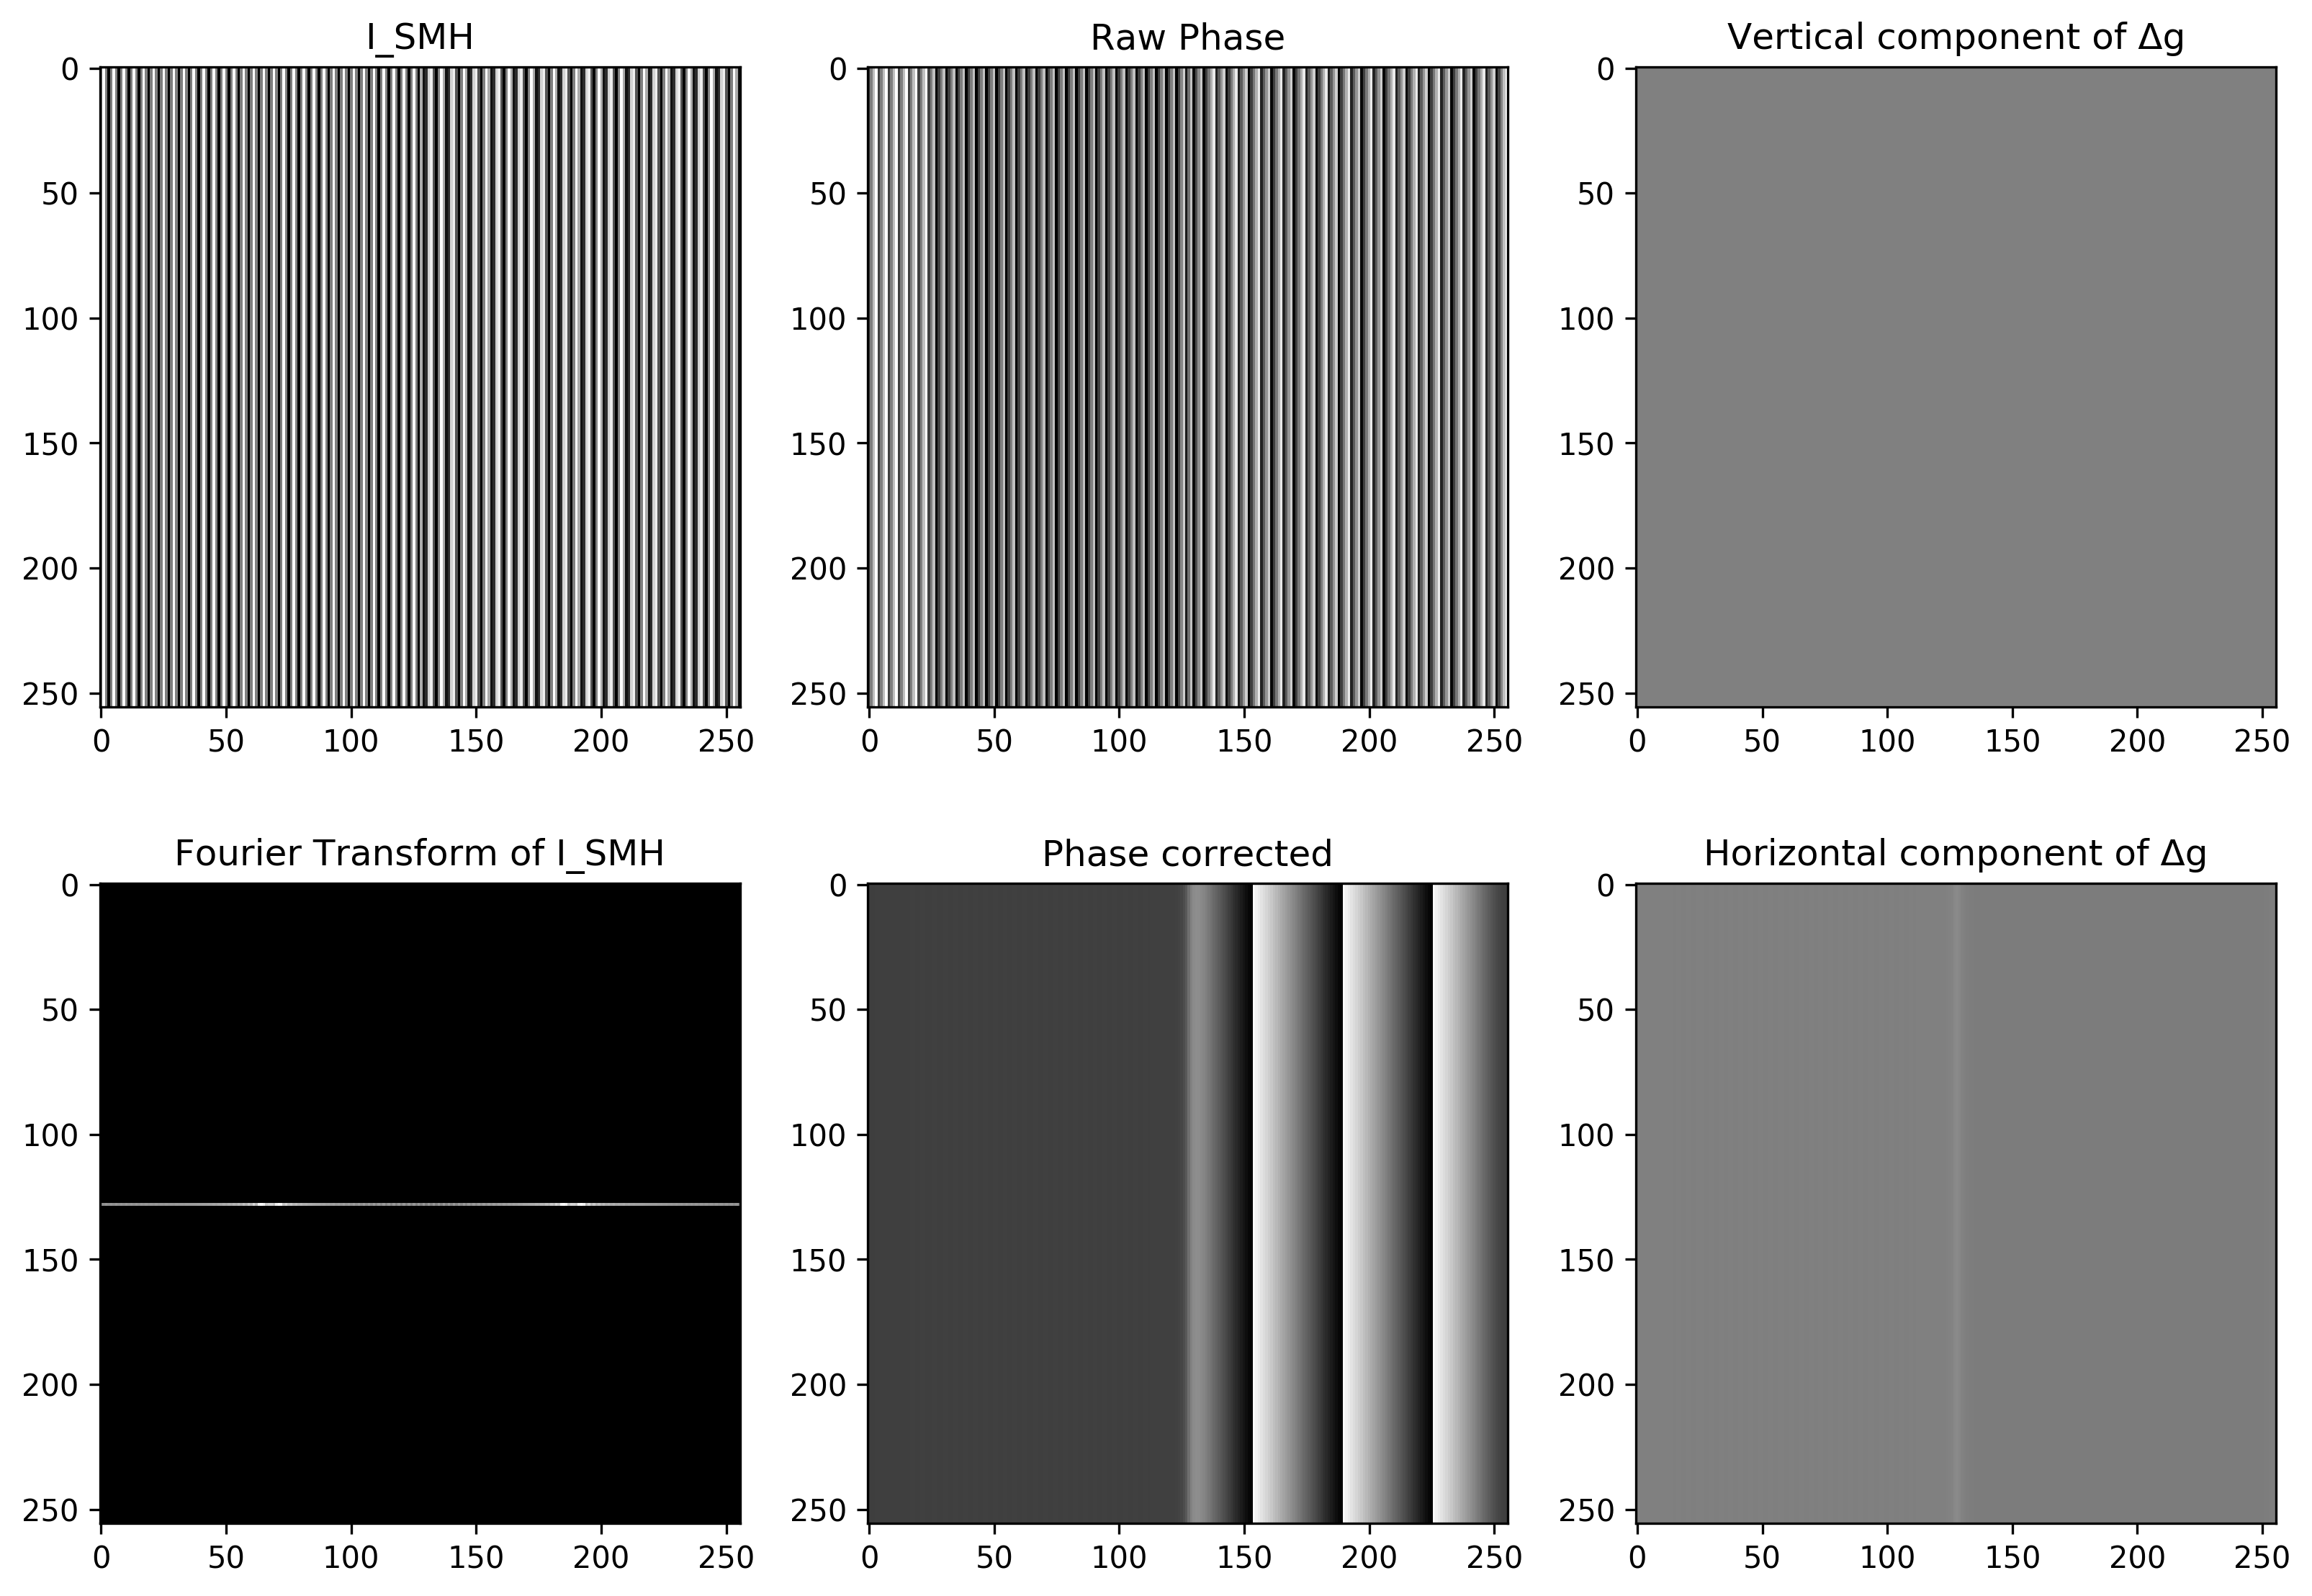
\includegraphics[scale=0.5]{Figures/Test_3_explanation.png}
\caption{Visual representation of one test case for \cref{Test_Report_3}}
\label{fig:Test_3_explanation}
\end{center}
\end{figure}

As done in \cref{Test_Report_2}, it is possible to slice the dataset to represent a 1D profile because the periodicity and the strain is only generated along the horizontal axis. The 1D data visualization is done in \cref{fig:Test_3_explanation_1D}. The presence of two different periodicities is confirmed in both the I{\_}SMH and the Fourier Transform of I{\_}SMH plots. Two areas with their own frequencies are clearly observable. Again similar spreading in frequency of the Fourier Trasform of I{\_}SMH that in \cref{fig:Test_2_Test_cases} are highlighted. The phase corrected plot also shows two different regions with different behaviour. Because of the difference of frequency, the phase is constant on the left side and varying on the right side. These results are expected since the strain corresponds to the slope of the phase. Therefore, with a flat phase, no strain is expected and with a varying phase, a strain is expected. The value of the slope is directly linked to the strength of the strain. The final output $\overrightarrow{\Delta g}$ is confirming a strain observed on the right side of the profile. There is an important spike on the interface between the unstrained and strain region but this is a known weakness of GPA algorithm. One assumption is to not have an abrupt variation of phase in order to model the derivative of the phase as the variation of the wave vector $\overrightarrow{g}$. Any interface won't respect this hypothesis and it is only possible to limit the spiking effect by playing with the mask parameters.

\begin{figure}[H]
\begin{center}
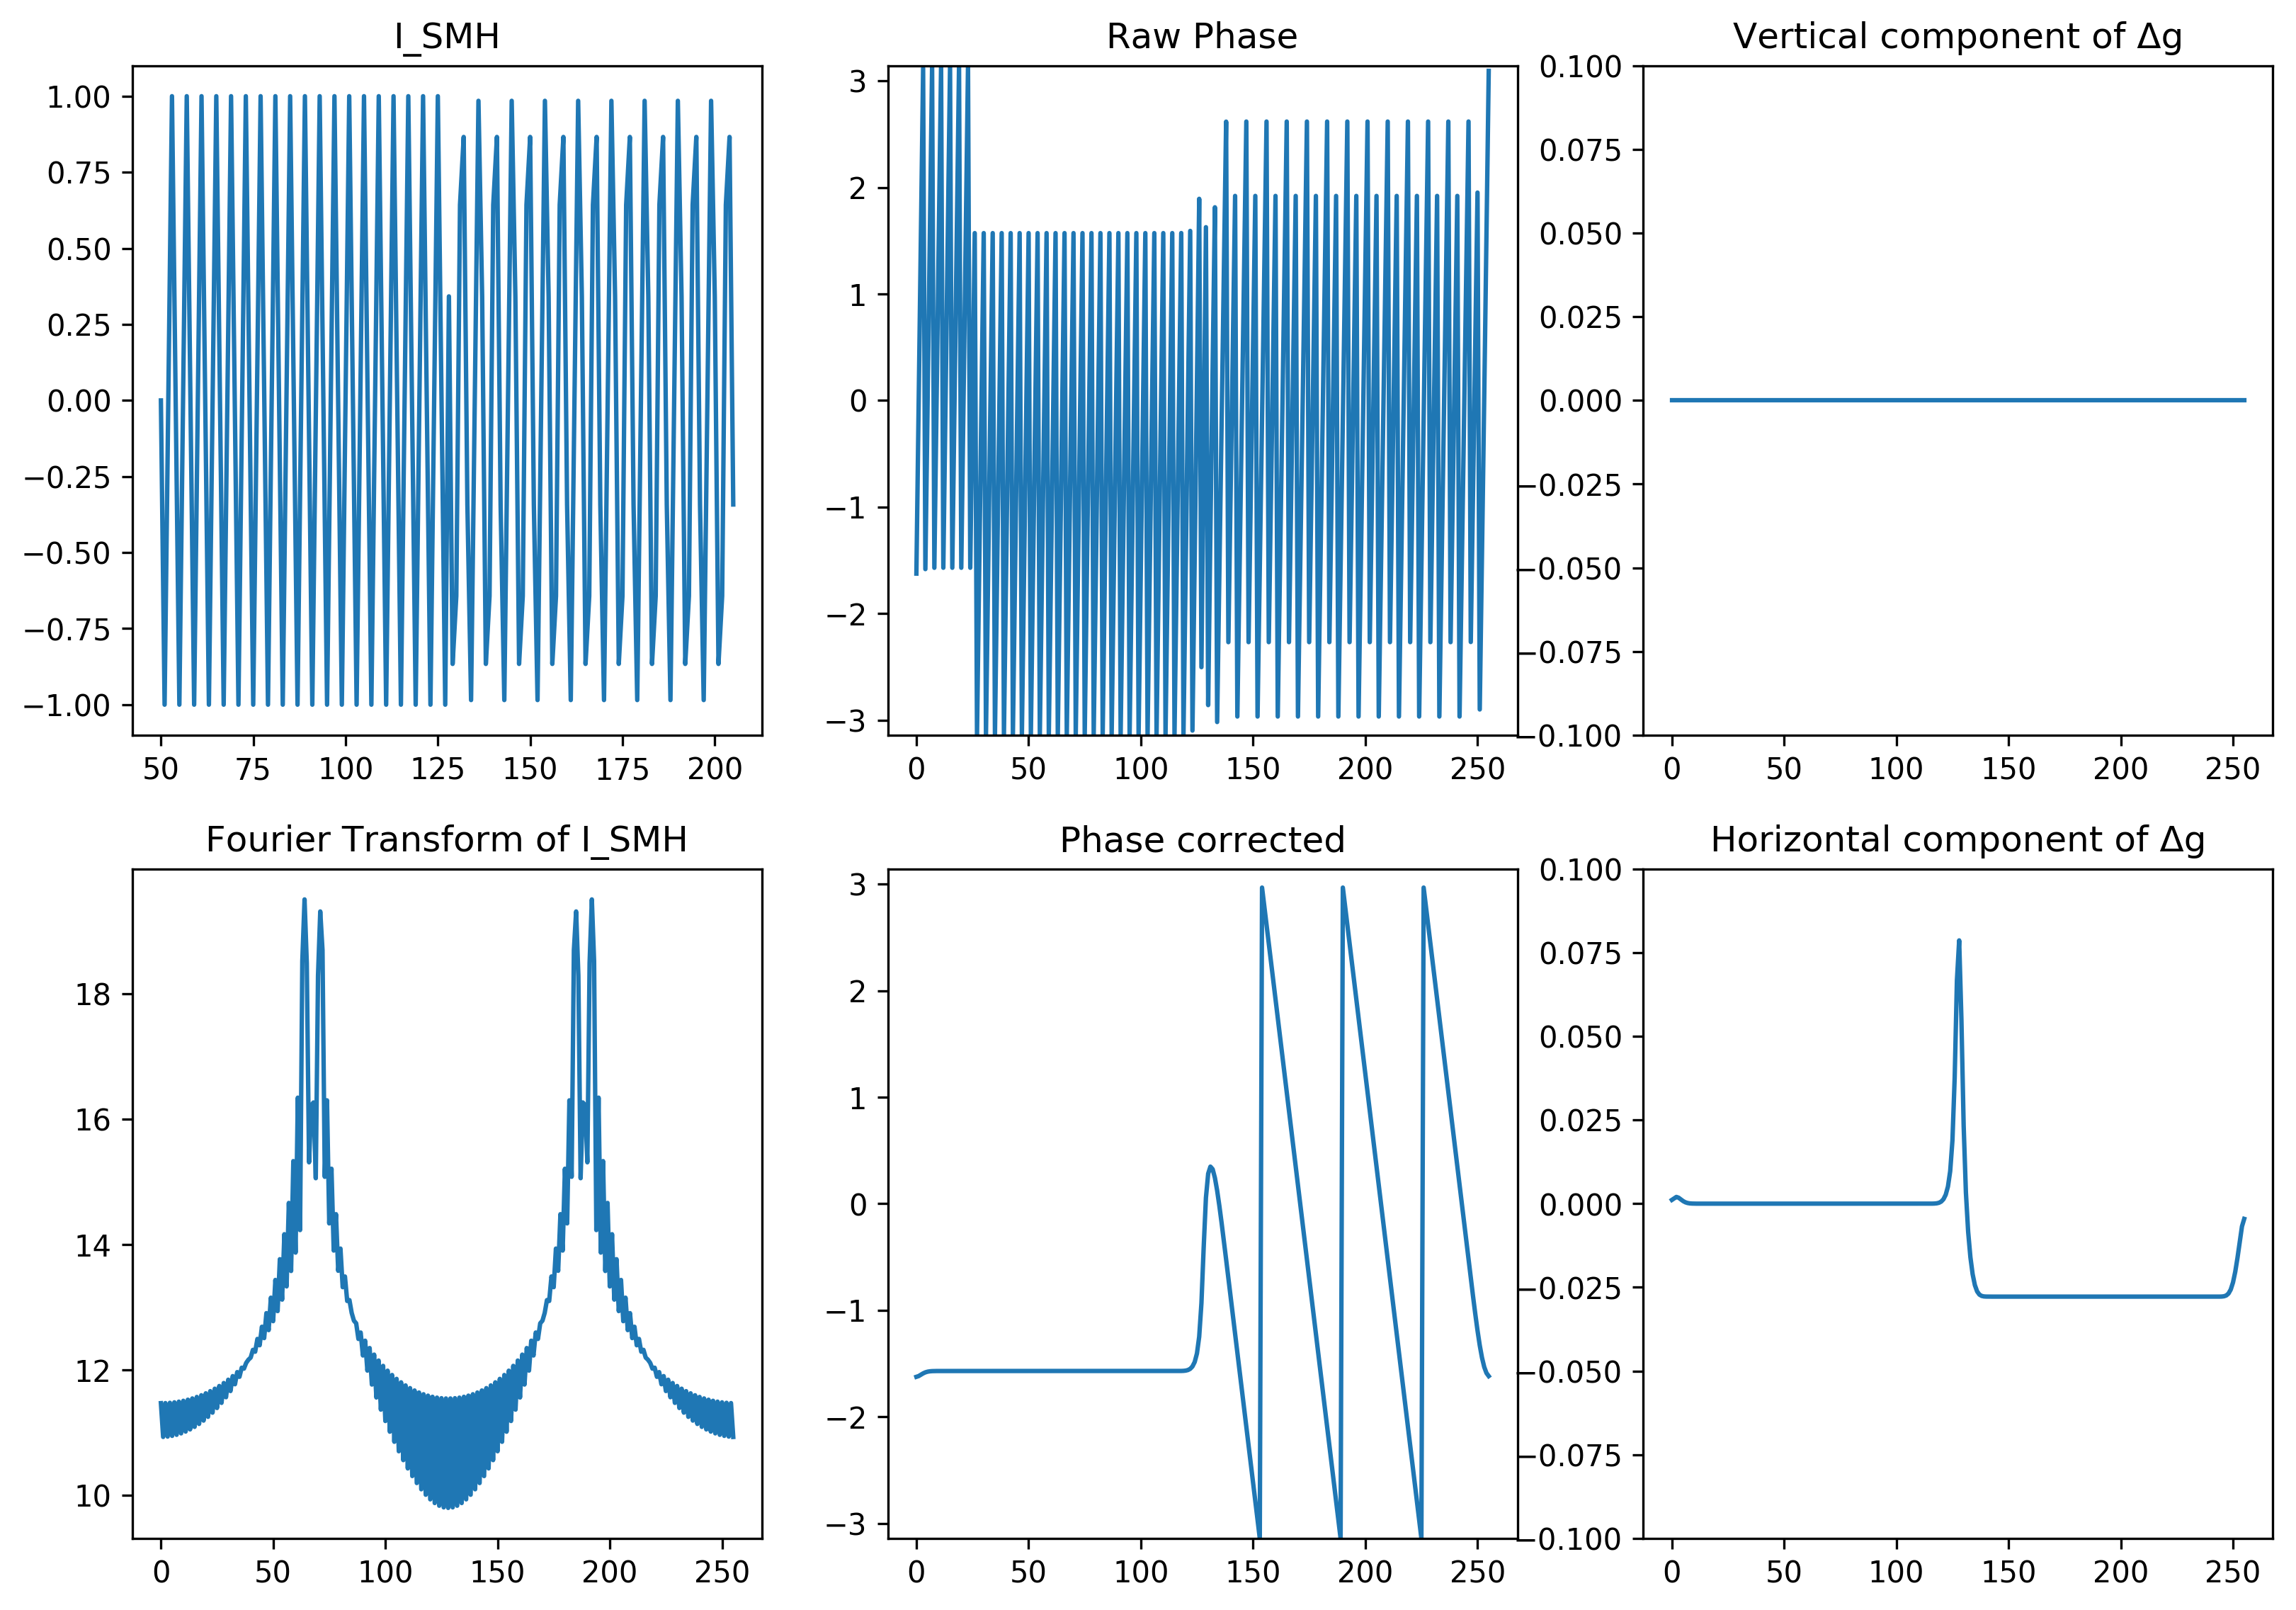
\includegraphics[scale=0.5]{Figures/Test_3_explanation_1D.png}
\caption{1D visual representation of one test case for \cref{Test_Report_3}}
\label{fig:Test_3_explanation_1D}
\end{center}
\end{figure}

To check the performance of the GPA algorithm the error between the input strain and the output strain can be calculated. Results are shown in \cref{tb:Metric_test_3_single_case} and the error seems to be on the same order of magnitude as the standard deviation of the worst case in \cref{Test_Report_2}.

\begin{table}[H]
\centering
\begin{tabular}{|c|c|c|}
\hline
$\overrightarrow{g} \ \text{(pixel)}$ & $\overrightarrow{K} \ \text{(pixel)}$ & $\text{Error}=|\overrightarrow{\Delta g}_{\text{sim}}-\overrightarrow{\Delta g}_{\text{gpa}}| \ \text{(pixel)}^{-1}$ \\
\hline
4 & 4.5 & 5.55555637e-02 \\ \hline
\end{tabular}
\caption{Table of metrics on one test case for \cref{Test_Report_3} }\label{tb:Metric_test_3_single_case}
\end{table}

Several test cases can be designed to see if the error is evolving with the level of strain. The following periodicities on the right side of the image have been tested to verify the GPA algorithm : 3, 3.8, 3.9, 4, 4.1, 4.2 and 5 pixels. The test cases should respectively display the following level of strain : 1/4 - 1/3, 1/4 - 1/3.8, 1/4 - 1/3.9, 0, 1/4 - 1/4.1, 1/4 - 1/4.2 and 1/4 - 1/5 $\text{pixel}^{-1}$. The results of the tests are highlighted in \cref{fig:Test_3_test_results} and in the table \cref{tb:Metric_test_3_multi_case}. 

\begin{figure}[H]
\begin{center}
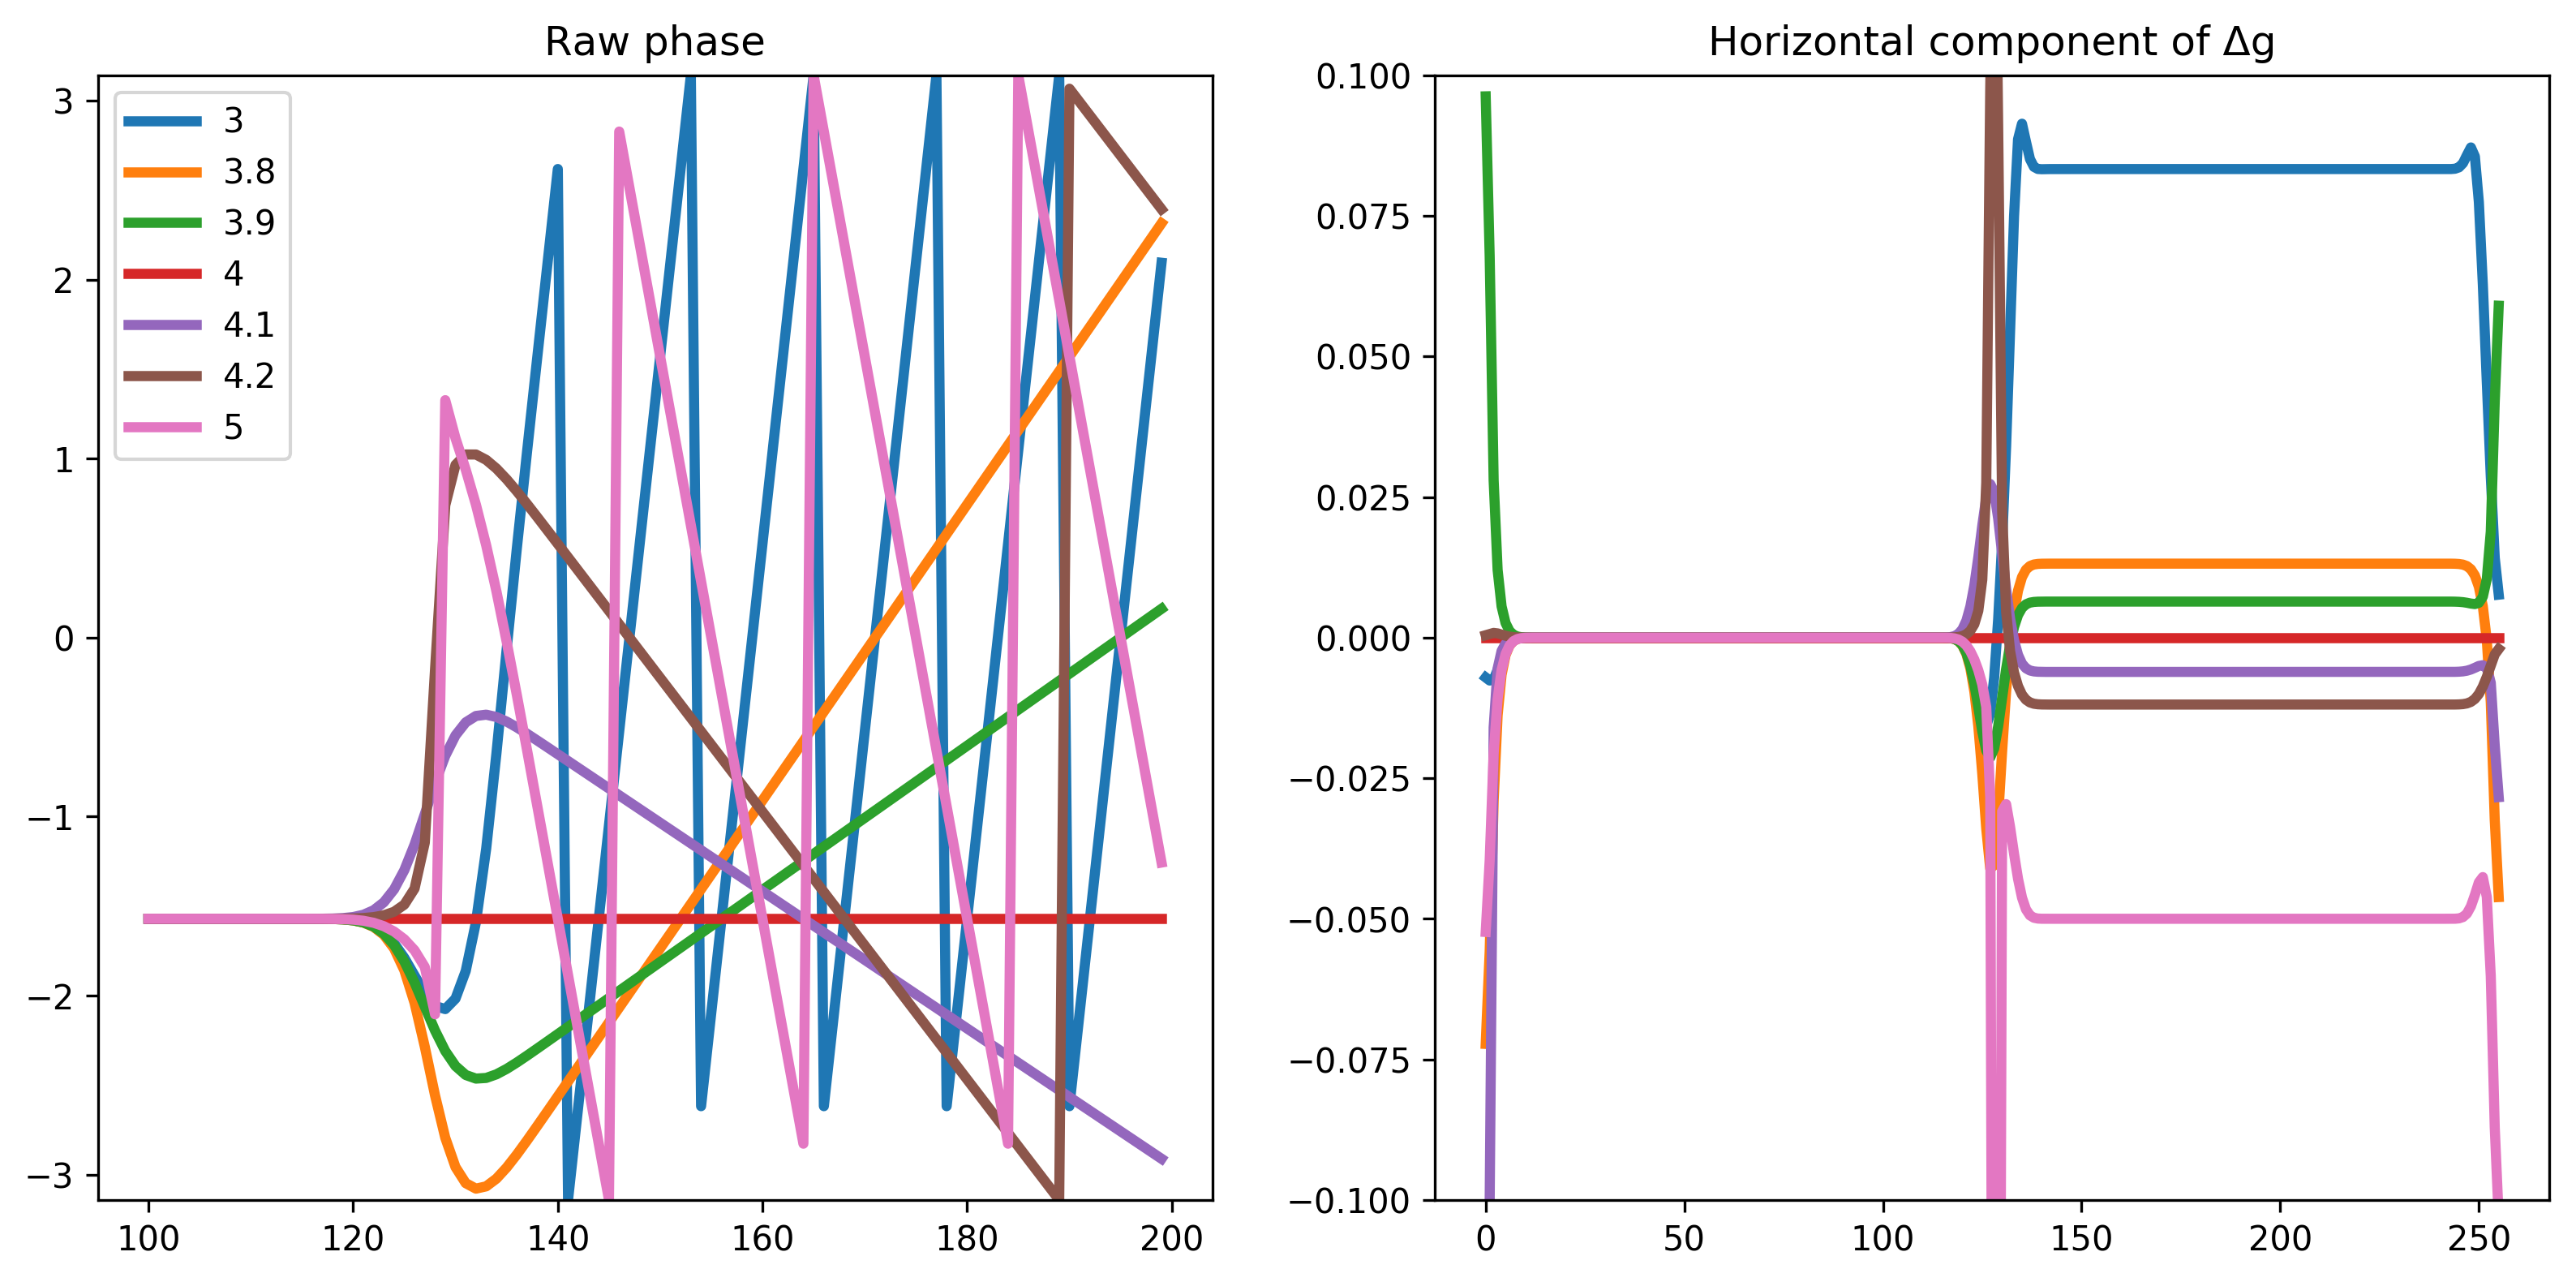
\includegraphics[scale=0.5]{Figures/Test_3_test_results.png}
\caption{1D visual representation of the test results for all the cases tested in \cref{Test_Report_3}}
\label{fig:Test_3_test_results}
\end{center}
\end{figure}

\begin{table}[H]
\centering
\begin{tabular}{|c|c|c|}
\hline
$\overrightarrow{g} \ \text{(pixel)}$ & $\overrightarrow{K} \ \text{(pixel)}$ & $\text{Error}=|\overrightarrow{\Delta g}_{\text{sim}}-\overrightarrow{\Delta g}_{\text{gpa}}| \ \text{(pixel)}^{-1}$ \\
\hline
4 & 3 & 1.66666626e-01 \\ \hline
4 & 3.8 & 2.63157758e-02 \\ \hline
4 & 3.9 & 1.28205175e-02 \\ \hline
4 & 4 & 8.32667268e-16 \\ \hline
4 & 4.1 & 1.21951224e-02 \\ \hline
4 & 4.2 & 2.38095207e-02 \\ \hline
4 & 5 & 9.99999872e-02 \\ \hline
\end{tabular}
\caption{Table of metrics for all the cases tested for \cref{Test_Report_3}}\label{tb:Metric_test_3_multi_case}
\end{table}

The error seems to increase slowly with the level of strain. Nevertheless, the higher the level of strain, the higher the radius of the mask should be. In this case, we kept the radius of the mask constant which can be at the disadvantage of higher strain level. The effect of the mask radius should be also assessed to give a more complete picture of the error evolution.
\end{TestRep}

\section{Nonfunctional Requirements Evaluation}

Nonfunctional Requirements have not been addressed for the moment.
	
\section{Comparison to Existing Implementation}	

No other equivalent open-access software has been identified for a comparison. sMoir{\'e} program (available on \href{https://www.hremresearch.com/}{HREM website}) is a good candidate but a licence must be bought in order to use the software. The licence purchase is not an option, moreover all aspects of \progname{} are not covered by sMoir{\'e}.

The GPA algorithm used in \progname{} could be however compared to other open-access GPA software and is planned to be performed. Nevertheless, most of them are plug-ins for Digital Micrograph software therefore an interface must be designed to perform a comparison with \progname{}. 

\section{Unit Testing}

A couple of unit tests were performed in order to verify the proper behaviour of a few functions. The amount of tests are still not sufficient to qualify the reliability of \progname{} nevertheless, the Data Structure Module has been tested such as a few properties of the Mask module. The test can be run using pytest testing framework and the content of the test can be found in the python files with the designation test{\_}*.py (the * replacing the name of the module tested).

\section{Changes Due to Testing}

A new mask function has been implemented called mask{\_}gaussian because of the poor performance of the mask{\_} classic function (very noisy data). The results of the test with the classic mask will be discussed in the future.

\section{Automated Testing}

For the moment, only a manual testing approach has been considered.

\section{Trace to Requirements}

Not enough tests have been performed to assess the requirement of \progname{}.
		
\section{Trace to Modules}

Not enough tests have been performed to assess the proper behaviour of the modules in \progname{}.		

\section{Code Coverage Metrics}

N/A

\bibliographystyle{ieee}

\bibliography{TestReport}

\end{document}